\section{Tutorial Resources}
\label{sec:Resources}

	Below are some top sources guides and tutorials for the Raspberry Pi 
	
	\subsection{Raspberry Pi Tutorials}
	
		\subsubsection*{Raspberry Pi Resources}
	
			\url{https://www.raspberrypi.org/resources/}
			\begin{center}
				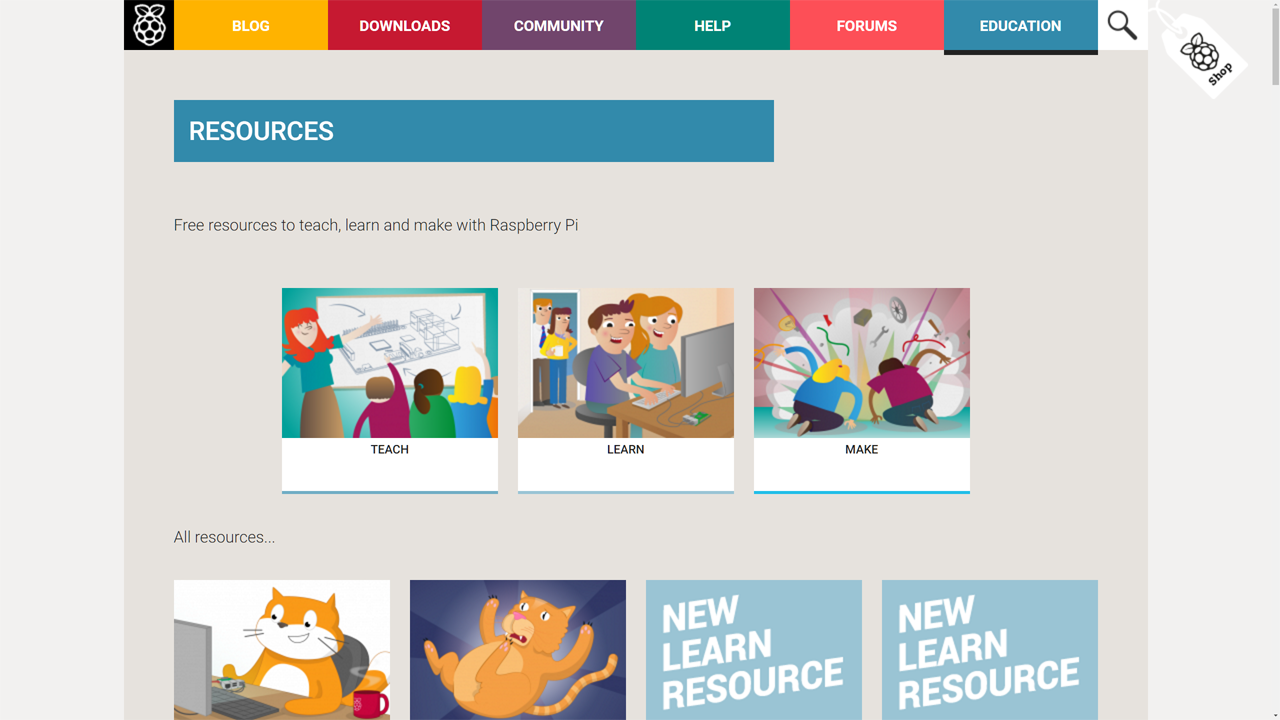
\includegraphics[width=0.5\linewidth]{sections/2_Resources/raspberrypiorg}
			\end{center}

	
			The official Raspberry Pi website should be your first stop, it's chock full of introduction tutorials and project ideas for most of the software we've covered today.
	
		\subsubsection*{The MagPi Magazine}
	
			\url{https://www.raspberrypi.org/magpi/}
			\begin{center}
				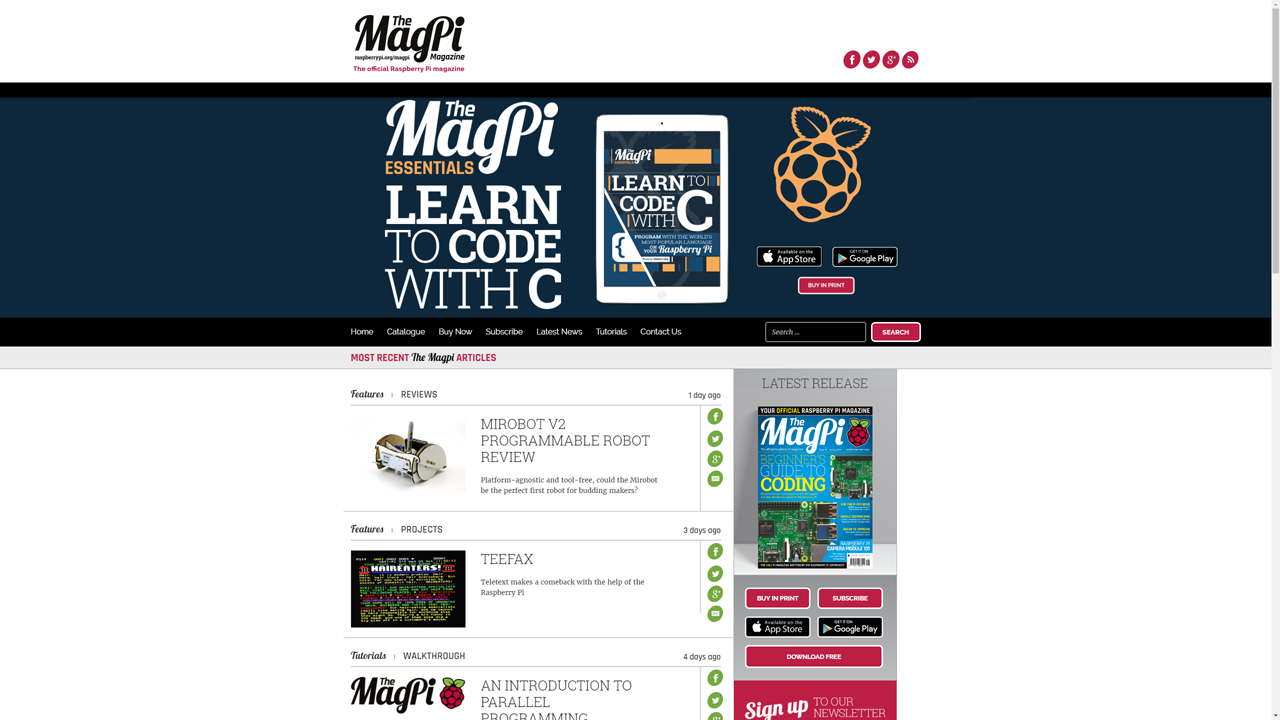
\includegraphics[width=0.5\linewidth]{sections/2_Resources/magpi}
			\end{center}		
				
			The MagPi started as a community run print magazine for the Raspberry Pi, and has now become the official magazine of the Raspberry Pi.
			
			Available in print (can be found in many supermarkets), or as a free download, each one is filled with articles, features and tutorials, all for the Raspberry Pi.
			
		\subsubsection*{The Raspberry Pi Guy}
			
			\url{http://www.theraspberrypiguy.com/tutorials/}
			\begin{center}
				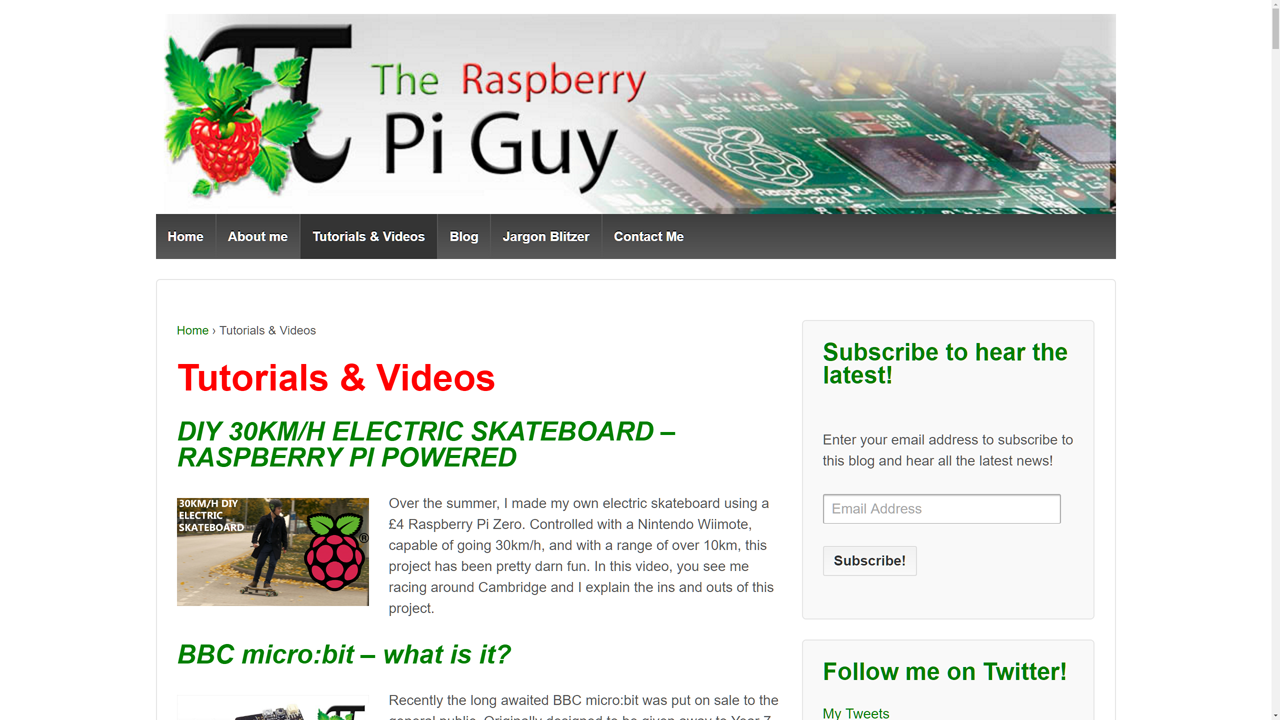
\includegraphics[width=0.5\linewidth]{sections/2_Resources/piguy}
			\end{center}	
			
			Matt was one of the first people to start producing regular video content for the Raspberry Pi, he was only 12 when the Pi was first released!
			
			Every few months, he produces a new video tutorial, showing off cool projects and uses for the Raspberry Pi, covering things as wide as Steam game streaming, robotics, or even building an electric skateboard.
		
	\subsection{Programming Language Tutorials}
	
		Ready to stretch your legs and try another programming language? Here are some quality tutorials for learning some new languages.
		
		\url{https://www.codecademy.com/learn/learn-java}
		
		Java has big long lines of code which look scarier than they are, but it's a great second language to learn, and a great introduction to object orientated programming.
		
		\textit{We'll have more here on the online version of these notes soon. In the meantime, why not ask us at today's Pi Clinic? We'll be able to find and recommend books and online tutorials for anything you might like to learn.}
	
		
	
\iffalse
	
		Ready to stretch your legs and try another programming language? Here are some quality tutorials for learning some new languages.
		
		\subsubsection*{If you want to try something else:}
		
			\url{https://www.codecademy.com/learn/learn-java}
			
			Java has big long lines of code which look scarier than they are, but it's a great second language to learn, and a great introduction to object orientated programming.
		
		\subsubsection*{If you're feeling brave:}
		
			\url{http://www.learn-c.org/}
			
			C is 45 years old. It's one of the oldest programming languages still in use, but with good reason.
			
			It's a familiar language syntax to things like Java, and pointers provide a challenge that's difficult to grasp at first, but very rewarding.
	
		\subsubsection*{If you're feeling foolhardy:}
		
			\url{http://www.learncpp.com/}
			
			Linus Torvalds and a few others may disagree, but C++ aimed to build on the foundations of C.
			
			This language will provide a challenge, but it's one of the most widely used programming languages there is. You can even use it to jump off into things like graphics rendering (\url{https://learnopengl.com/})
		
		\subsubsection*{If you're just feeling silly, now:}
		
			\url{https://www.codecademy.com/learn/php}
			
			A scary looking syntax, but PHP forms the majority of server-side code on the modern web. If you're already planning far ahead for a move into web development, you'll want to learn some PHP.
		
		\subsubsection*{If you want to build web apps:}
		
			\url{https://www.codecademy.com/learn/learn-javascript}
			
			If you want your webpages to do more than just display text, Javascript is the most common programming language used in the web today.
			
			Once you've learnt the basics, you'll 
\fi